\documentclass{article}
\usepackage{graphicx} % Required for inserting images
\usepackage[ruled,vlined]{algorithm2e}
\usepackage{xcolor} % for colored text
\usepackage{graphicx} % for including graphics
\usepackage{amsmath} % for advanced math features
\usepackage{float}
\usepackage{amssymb}
\usepackage{amsthm}

\title{CS529 Project 1 Report - Group 15}
\vspace{3cm}
\author{
    \begin{tabular}[t]{c@{\hskip 2em}c} % Two columns with some space in between
        Behnoud Alaghband & Zhuoming Liu  \\
        University of New Mexico & University of New Mexico \\
        \texttt{balaghband@unm.edu} & \texttt{dawnmoon@unm.edu}
    \end{tabular}
}


\begin{document}

\maketitle

\section{Data}
\subsection{Data Overview}
The dataset is a 472432 $\times$ 27 matrix, 472432 records and 27 features (columns). Among 27 features, there are 25 explanatory features, 1 target feature ("isFraud"), 1 index feature ("TransactionID"). Except the target feature and index feature, the rest 25 features are classified as numerical or categorical (Table 1).

\begin{table}[H]
    \centering
    \resizebox{1 \textwidth}{!}{
        
        \begin{tabular}{r|r|r|r|r}
            Feature & Numerical & Categorical & \# of Unique values & \% of missing values \\\hline
            ProductCD& & \checkmark & 5 & 0\\
            card1& &\checkmark &12815 & 0\\
            card2& &\checkmark &501 & 1.52\\
            card3& &\checkmark &112 & 0.27\\
            card4& &\checkmark &5 & 0.27\\
            card5& &\checkmark &115 & 0.72\\
            card6& &\checkmark &5 & 0.27\\
            addr1& &\checkmark &304 & 11.09\\
            addr2& &\checkmark &72 & 11.09\\
            c1&\checkmark &&1350 & 0\\
            c2&\checkmark &&1064 & 0\\
            c3&\checkmark &&21 & 0\\
            c4&\checkmark &&1078 & 0\\
            c5&\checkmark &&319 & 0\\
            c6&\checkmark &&1158 & 0\\
            c7&\checkmark &&914 & 0\\
            c8&\checkmark &&1002 & 0\\
            c9&\checkmark &&204 & 0\\
            c10&\checkmark &&987 & 0\\
            c11&\checkmark &&1210 & 0\\
            c12&\checkmark &&927 & 0\\
            c13&\checkmark &&1393 & 0\\
            c14&\checkmark &&1018 & 0\\
            TransactionAmt&\checkmark &&7898 & 0\\
            TransactionDT&\checkmark &&461340 & 0\\
        \end{tabular}
    }
    \caption{\label{tab:1} Data overview}
\end{table}
'TransactionDT' has 461340 unique values in our dataset (Table 1), indicating 'TransactionDT' should not be used in the decision tree (DT). Same reason from Micheal's book, 'TransactionDT' can cause a highly over-fitting tree. In fact, 'TransactionDT' is the date of transaction, usually meaningless for determining whether the transaction is fraud or not. Although an organization is faking the transaction in a particular day may happen in some cases, we don't take that situation into consideration. We will ignore 'TransactionDT' when building our Random Forest (RF).

\subsection{Records with "NaN"}
Some records have missing values for a certain feature. Table 2 gives out how many records have missing values in each feature. For example, there are 11.09\% of records have missing values in "addr2" feature.\\
Two strategies were applied in the training phase.
\begin{enumerate}
    \item Remove records
    \\We removed the record if any of its features has a missing value. After the data cleaning, we had 87.17\% records left for use. Obviously, this strategy is very easy for implementation, but it resulted in less data in the training phase, which affected the performance of RF.
    \item Simulate feature value
    \\For the record with a missing feature, we will assign it with the most common feature value from the rest of the dataset. This can keep our records as much as possible. And We won't waste those useful information from the records with missing values. Actually based on Table 1, we can simulate an extremely worst case -- one record has 7 missing feature values (card2 -card6, addr1, addr2). The rest 18 features contain useful information still.
\end{enumerate}
Among these 2 strategies, we prefer to use the $2^{nd}$ one.\\\\
In validation phase, we are using a different strategy. We will try every possible values and gave predictions, among which we select the most frequent one as our final prediction. This is the same strategy we are using when the DT sees an un-seen feature value in training pahse.\\\\
For example, given a tree and a to-be-predicted record (Fig 1). The root node of this DT is "ProductCD" with 4 sub-branches. Only branches "W" and "D" has a child-node "C1" and "card1" respectively. In the training phase, This DT only sees "5812", "4472" and "9633" for "card1" feature.\\\\  
In the to-be-predicted record, the feature "ProductCD" is a missing value ("NaN"), "C1" is 50 and "card1" is "17399" (other features are ignored in this example). When the DT do the prediction, it will first scan the value of "ProductCD". Becasue it is "NaN", so it will travelse each sub-branch. 
\begin{itemize}
    \item \textbf{sub-branch 1} $ProductCD = W \land C1 = 50\rightarrow Target = Fraud$
    \item \textbf{sub-branch 2} $ProductCD = H \rightarrow Target = Fraud$
    \item \textbf{sub-branch 3} $ProductCD = R \rightarrow Target = NotFraud$
    \item \textbf{sub-branch 4} $ProductCD = D \land$
    \begin{itemize}
        \item \textbf{sub-branch 4.1} $card1 = 5812 \rightarrow Target = Fraud$
        \item \textbf{sub-branch 4.2} $card1 = 4472 \rightarrow Target = NotFraud$
        \item \textbf{sub-branch 4.3} $card1 = 9633 \rightarrow Target = NotFraud$
    \end{itemize}
\end{itemize}
Because this DT never sees the value of "card1 = 17399" in the training phase, it will travelse every possible values in sub-branch under the node "card1". \\\\
In the end this DT predicts a list of potential values as [Fraud, Fraud, NotFraud, Fraud, NotFraud, NotFraud]. We have 3 "Fraud" and 3 "NotFraud". Because the number of times "Fraud" occurred was at least half, we assign the final prediction as "Fraud" ("NotFraud" less than half time).

\begin{figure}[H]
  \centering
  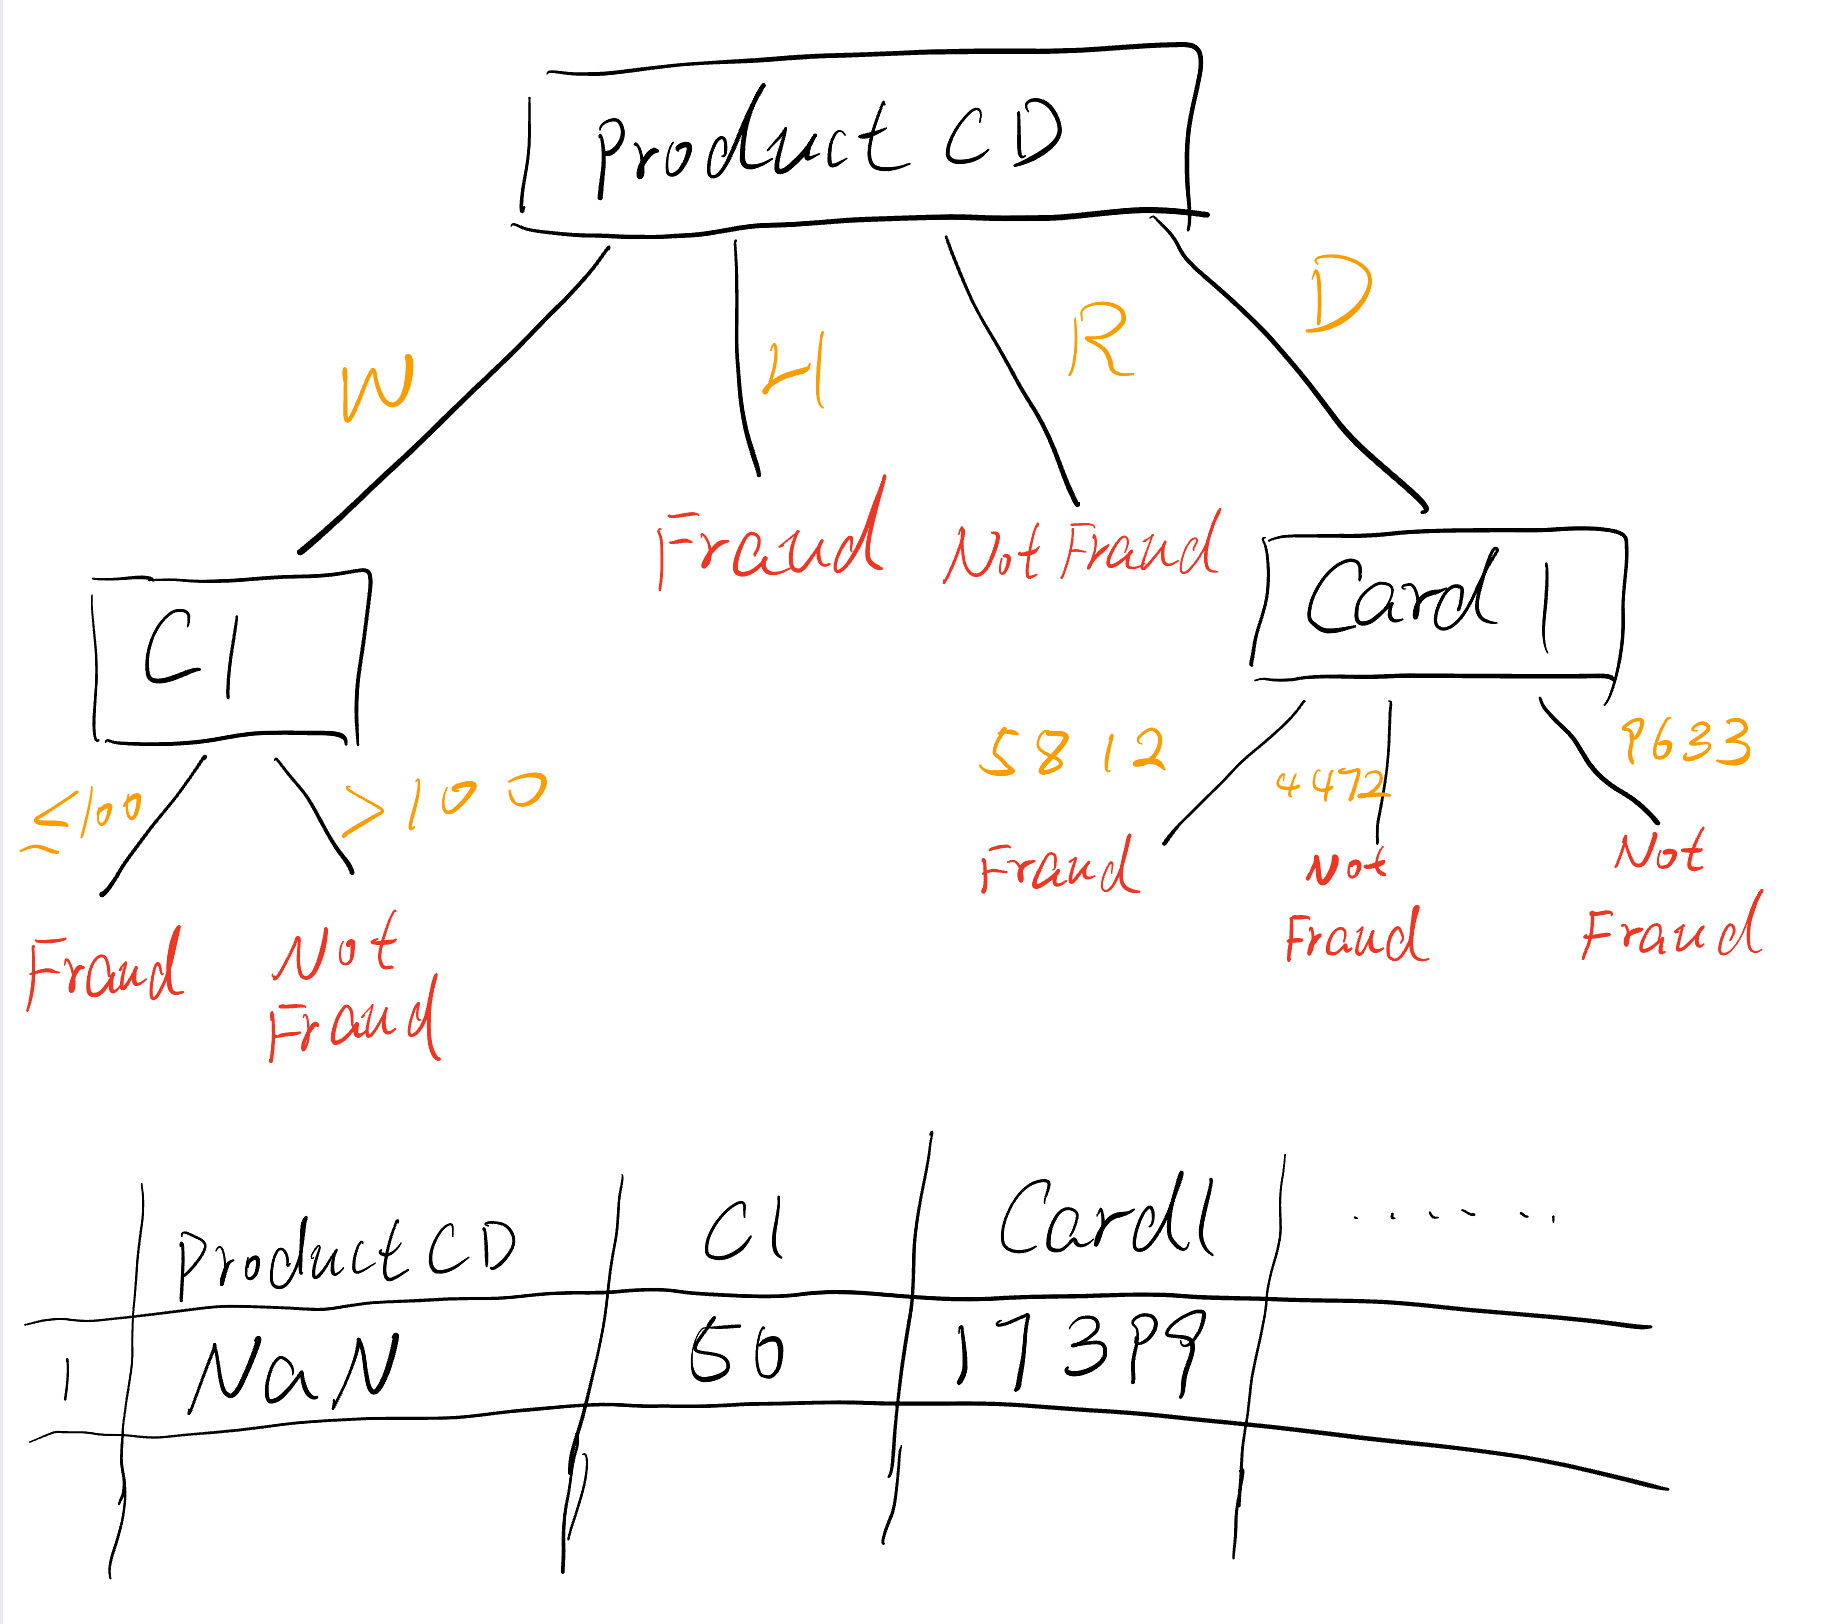
\includegraphics[width=1\linewidth]{Fig/NaN_test.jpeg}
  \caption{\label{fig:1}A demo of 1 DT and 1 record}
\end{figure}


\subsection{Imbalanced data}
The dataset has 96.5\% of \textbf{not Fraud} transaction records, which is a significantly imbalanced (Table 2). To guarantee that each DT has enough \textbf{Fraud} transaction records while we randomly select 80\% of data in the training phase, we first split our dataset into "positive" set (Fraud) and "negative" set (Not Fraud). Then we extract 80\% from both sets as our training set, and the left 20\% as our validation set (Fig 2). By doing so, the algorithm is able to see a certain number of "Fraud" data in training phase, and have enough "Fraud" data for the validation phase.
\begin{table}[H]
    \centering        
    \begin{tabular}{r|r}
        Target & Percentage (\%)\\\hline
        Fraud& 3.50\\
        not Fraud& 96.50\\
    \end{tabular}
    \caption{\label{tab:2} Imbalanced target}
\end{table}
\begin{figure}[H]
  \centering
  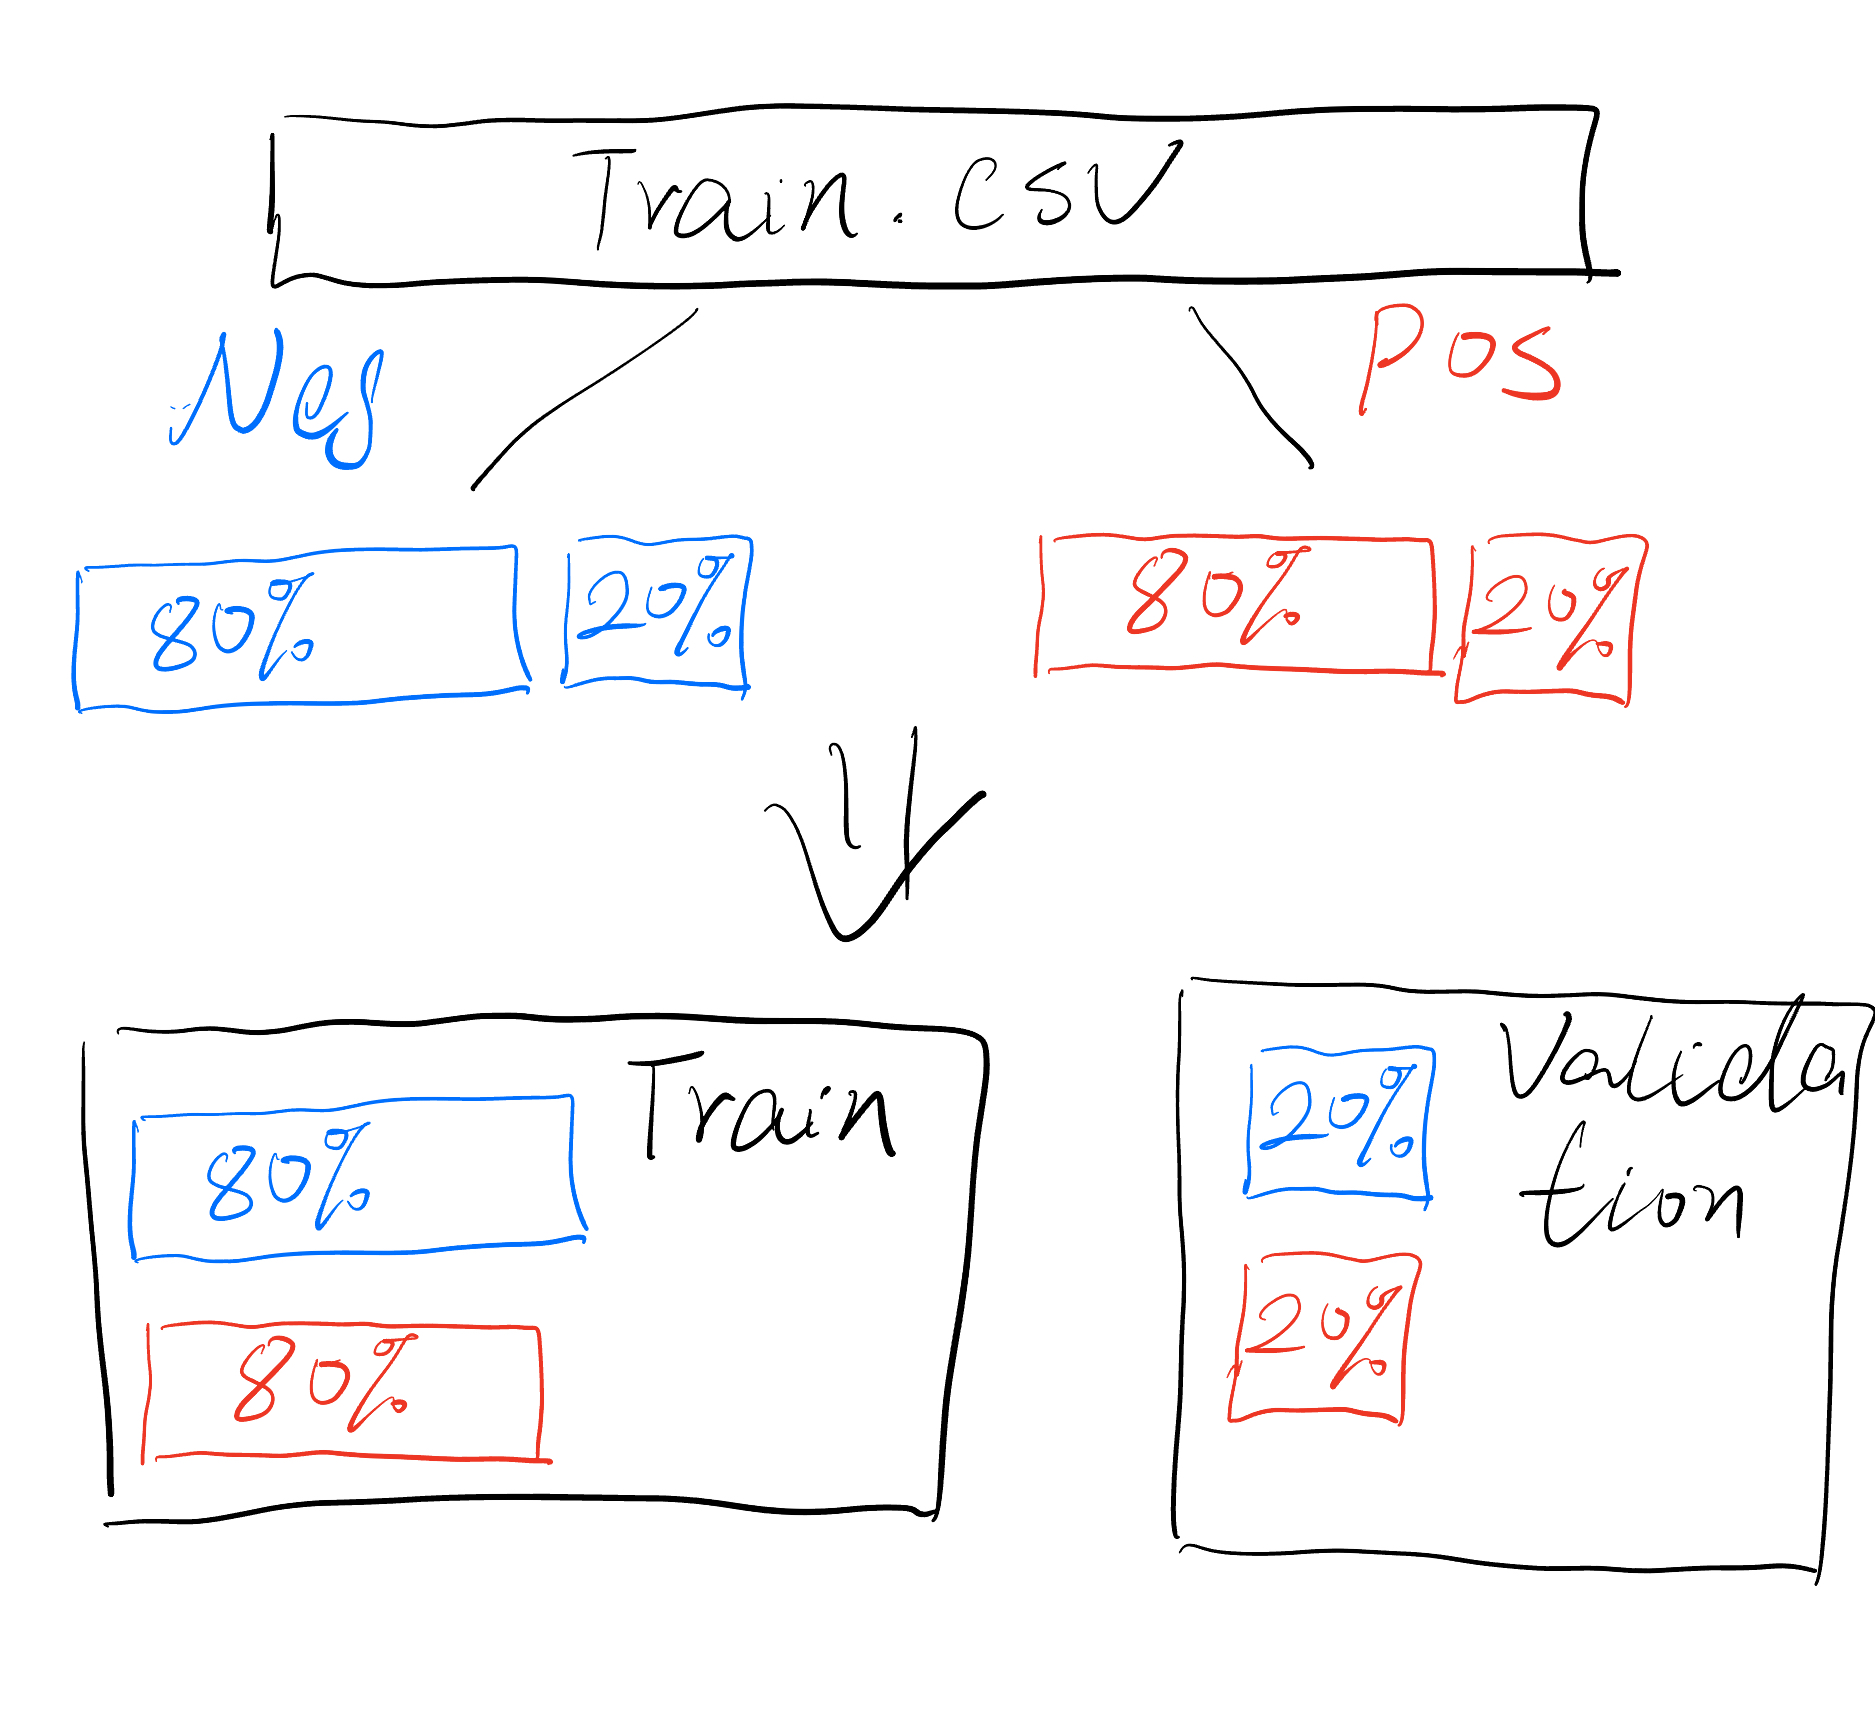
\includegraphics[width=1\linewidth]{Fig/Imblanced_data.jpeg}
  \caption{\label{fig:2}Splitting data strategy}
\end{figure}

\section{Information Gain}
we calculate information gain by Info-Gain function :

\begin{algorithm}[H]
\SetAlgoLined
\KwIn{Input\_Dataframe, Split\_feature, IG\_methods, Num\_Cat}
\KwOut{Information Gain}
\KwResult{Calculate Information Gain based on the given parameters}

\SetKwFunction{InfoGain}{Info\_Gain}
\SetKwProg{Fn}{Function}{:}{}

\Fn{\InfoGain{Input\_Dataframe, Split\_feature, IG\_methods, Num\_Cat}}{
    % Function body
}

\caption{Info\_Gain function}
\end{algorithm}

\textbf{Information gain function}

\begin{center}
\begin{tabular}{|c|c|p{7cm}|}
\hline
\textbf{Input Variable} & \textbf{Type} & \textbf{Definition} \\
\hline
\textcolor{green}{Input\_Dataframe} & \texttt{pandas.DataFrame} & This is your chosen subset of training data \\
\textcolor{green}{Split\_feature} & \texttt{String} & The chosen feature for calculating Information gain \\
\textcolor{green}{IG\_methods} & \texttt{String} & Three options: \textcolor{red}{Gini} for Gini index, \textcolor{red}{Entropy} for Max Entropy, \textcolor{red}{MisEr} for Miss classification\\
\textcolor{green}{Num\_Cat} & \texttt{String} & Two options: \textcolor{red}{Num} for a numeric feature, \textcolor{red}{Cat} for a categorical feature \\
\hline
\end{tabular}
\end{center}

This function has two possible returns: 

\begin{itemize}
    \item \textcolor{red}{[IG\_feature, Split point]}: if \textcolor{green}{Split\_feature} is a \textbf{numeric} feature
        \begin{itemize}
            \item \textbf{IG\_feature}: single float variable representing \textbf{Information Gain} of \textcolor{green}{Split\_feature}
            \item \textbf{Split point}: single float variable, the best binary split point for this numeric feature \textcolor{green}{Split\_feature}
        \end{itemize}
    \item \textcolor{red}{[IG\_feature, -3.14]}: if \textcolor{green}{Split\_feature} is a \textbf{categorical} feature
        \begin{itemize}
            \item \textbf{IG\_feature}: same as previous
            \item \textbf{-3.14}: Meaningless, and not to be used in the future. Just to make this function work recursively.
        \end{itemize}
\end{itemize}


\section{Discussion on the different values for $\alpha$ in chi square}

$\alpha$ represents the significance level as the probability that a hypothesis is rejected when it is true. The common value for $\alpha$ is 0.05 which means if the probability of the value is less than 5\%, the null hypothesis is rejected and there is a statistical significance between the data that has been observed and frequencies that are expected. If $\alpha$ is 0.01, it means the probability that a true null hypothesis is rejected is decreased but otherwise, the probability that a false bull hypothesis is not being rejected increases. 
In our project, we have $\alpha$ as 0.05 and we have chosen feature classes based on the unique value of split features in our dataframe. Then, we calculated degrees of freedom by multiplying number of feature classes (as row) -1 and target (isFraud or is not Fraud as columns) -1. 



\section{Discussion wrt design decisions for: missing data, numerical features, class imbalance}
\section{Interpreting the results and provides insights into the various model performance}
\section{Insights into the relationship between features and the target variable}


\end{document}
